\chapter{Design}
\label{ch:design}

Chapter~\ref{ch:methodology} described how the work was carried out. This chapter
describes what was built. It moves from the outside in: first the requirements the
system answers to and the shape they impose, then the containers the tool is made
of, then the modules inside the backend, the data they persist, and finally the
mechanism the whole thesis turns on --- the gated agentic retest loop. It closes
with the part of the design that is easiest to leave out of a dissertation and
most instructive to include: the architecture that was built, shipped, and then
deleted.

Every diagram in this chapter is generated from the project's own architecture
documentation rather than redrawn for the memoir. That is a deliberate
application of the docs-as-code rule of Section~\ref{subsec:docs}: a figure
copied by hand into LaTeX is a second description of the system, and the second
description is the one that silently goes stale.

\section{From requirements to design}
\label{sec:design-requirements}

The requirements were elicited in an interview at the start of the project and
recorded as a software-requirements specification, each with acceptance criteria
that a later change had to keep satisfying --- with four later requirements
(FR-16 to FR-19) added as recorded change requests as the retest model evolved.
Table~\ref{tab:requirements}
summarises them. The table is worth reading for its gaps as much as its entries:
of nineteen functional requirements, five no longer have an implementation, and
that is a design outcome rather than an omission --- Section~\ref{sec:design-evolution}
argues why.

\begin{table}[!htb]
\footnotesize
\renewcommand{\arraystretch}{1.25}
\begin{center}
\begin{tabular}{|L{1.5cm}|L{6.6cm}|L{4.4cm}|}
\hline
\rowcolor{tema!10}
\bft{Id} & \bft{Requirement} & \bft{Status in the delivered system} \\ \hline
FR-01 & Ingest PDF penetration-test reports & Implemented \\ \hline
FR-02 & Ingest structured reports (JSON/XML) & Implemented for JSON and manual entry; the XML door was not built \\ \hline
FR-03 & Extract structured findings with a language model & Implemented \\ \hline
FR-04 & Generate executable retest plans & \emph{Repurposed} as the user-owned retest goal \\ \hline
FR-05 & Human plan review and approval & \emph{Superseded} --- approval moved to every command \\ \hline
FR-06 & Target authorisation & Implemented, as network membership \\ \hline
FR-07 & HTTP probe executor & \emph{Deleted} with the batch path \\ \hline
FR-08 & Execution sanity checker & \emph{Deleted} with the batch path \\ \hline
FR-09 & Evidence-backed verdicts & Implemented \\ \hline
FR-10 & Full audit trail & Implemented, as an append-only transcript \\ \hline
FR-11 & Results dashboard (web interface) & Implemented \\ \hline
FR-12 & Machine-readable results export & Implemented \\ \hline
FR-13 & Pluggable language-model backends & Implemented \\ \hline
FR-14 & Browser-based probes & \emph{Dropped} --- subsumed by the sandbox \\ \hline
FR-15 & Evaluation harness & Implemented (harness; the evaluation run is future work) \\ \hline
FR-16 & Operator finding revision and annotation & Implemented \\ \hline
FR-17 & Interactive agentic retest console & Implemented \\ \hline
FR-18 & Reports chat assistant & Implemented \\ \hline
FR-19 & CVSS and MITRE ATT\&CK enrichment & Implemented; ground-truth tagging pending \\ \hline
NFR-01 & Verdict reliability & \emph{Not yet measured} --- the harness is built, the run is future work \\ \hline
NFR-02 & Full reproducibility & Replayable session transcript \\ \hline
NFR-03 & Safety (loopback only, no exposure) & Enforced by binding and topology \\ \hline
NFR-04 & Data protection & Satisfied by construction --- synthetic and lab data only \\ \hline
NFR-05 & Maintainability & Enforced by the gate of Section~\ref{sec:ci} \\ \hline
\end{tabular}
\end{center}
\caption[Requirements and their status in the delivered system]{The nineteen
functional and five non-functional requirements, and what became of each. Five
functional requirements --- FR-04, FR-05, FR-07, FR-08 and FR-14 --- were
implemented, tested and then removed or repurposed when the retest model changed;
they are discussed in Section~\ref{sec:design-evolution} rather than hidden.}
\label{tab:requirements}
\end{table}

Three requirements shape the architecture more than the rest, and it is worth
naming them before any diagram. FR-06 (only authorised targets are ever reached)
and NFR-03 (the tool is never exposed beyond the machine it runs on) are safety
constraints, and safety constraints are best met by structure rather than by
checks --- a theme returned to in Section~\ref{sec:design-runtime}. FR-10 (any
verdict must be traceable to the trail that produced it) is what forces the
persistence model of Section~\ref{sec:design-data}: a verdict cannot be a bare
row, it has to be a derivation of something append-only.

\section{Architectural overview}
\label{sec:design-overview}

\subsection{Context}

Figure~\ref{fig:arch-context} places the system among the actors and systems it
touches. There is exactly one human role --- the security auditor or developer
who wants to know whether previously reported findings are still exploitable ---
and exactly two external systems: a language-model backend, and the authorised
targets being retested.

\begin{figure}[!htb]
\centering
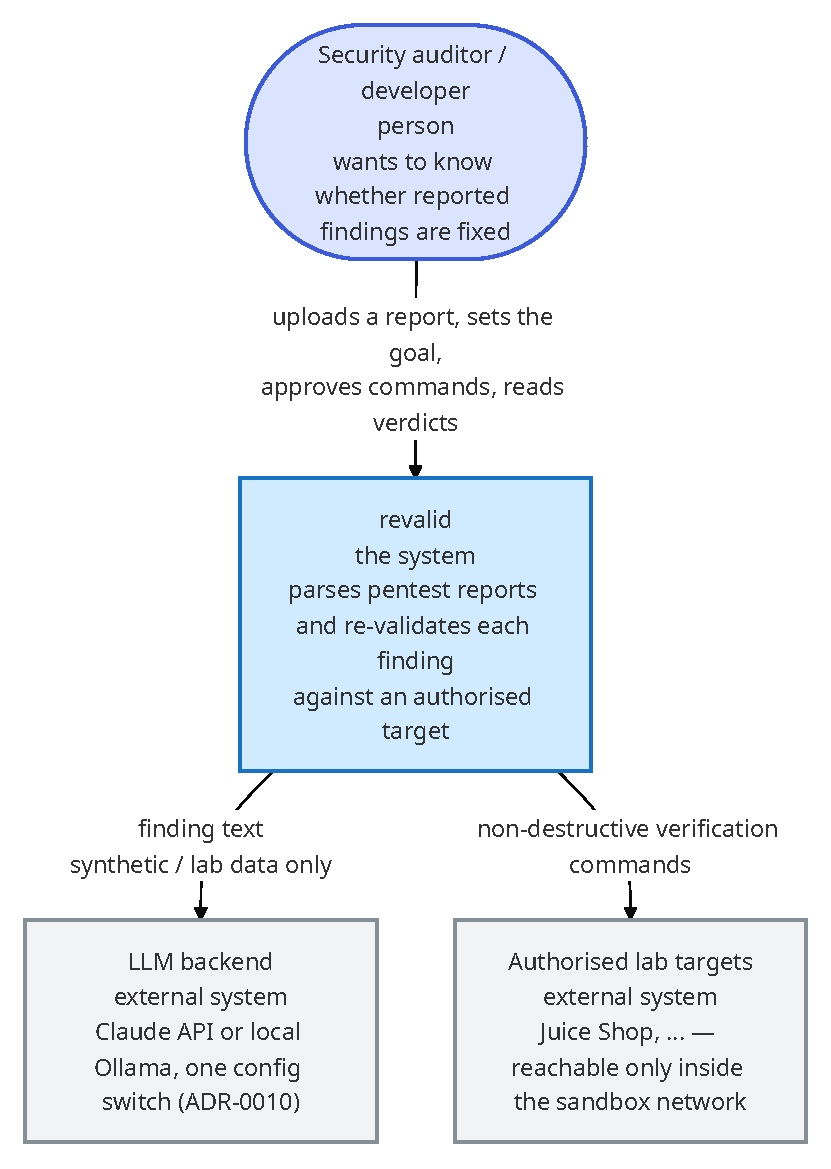
\includegraphics[width=0.62\textwidth]{figs/arch-context.pdf}
\caption[System context]{The system in its context. The auditor uploads a report,
sets a retest goal, approves commands and reads verdicts. The system sends finding
text to a language-model backend and non-destructive verification commands to the
authorised target --- and reaches that target only from inside the sandbox of
Section~\ref{sec:design-runtime}.}
\label{fig:arch-context}
\end{figure}

The narrowness of that context is itself a design decision. The tool has no
account system, no multi-tenancy, no notion of an organisation, and no
server-side deployment: it is a single-operator instrument, which is what makes
an approval gate on every command a reasonable interaction model rather than an
intolerable one. A tool used by ten people simultaneously could not ask a human
to approve each command; a tool used by one person during a focused revalidation
session can, and that is precisely the trade-off drawn in
Chapter~\ref{ch:sota}'s survey of autonomous testing agents.

\subsection{Containers}

Figure~\ref{fig:arch-containers} decomposes the system into its runnable parts.
The striking feature is how few there are. One \texttt{uvicorn} process serves
both the compiled single-page interface at the root and the JSON API beneath
\texttt{/api}; long-running work is handed to background tasks in the same
process; durable state is a single SQLite file.

\begin{figure}[!htb]
\centering
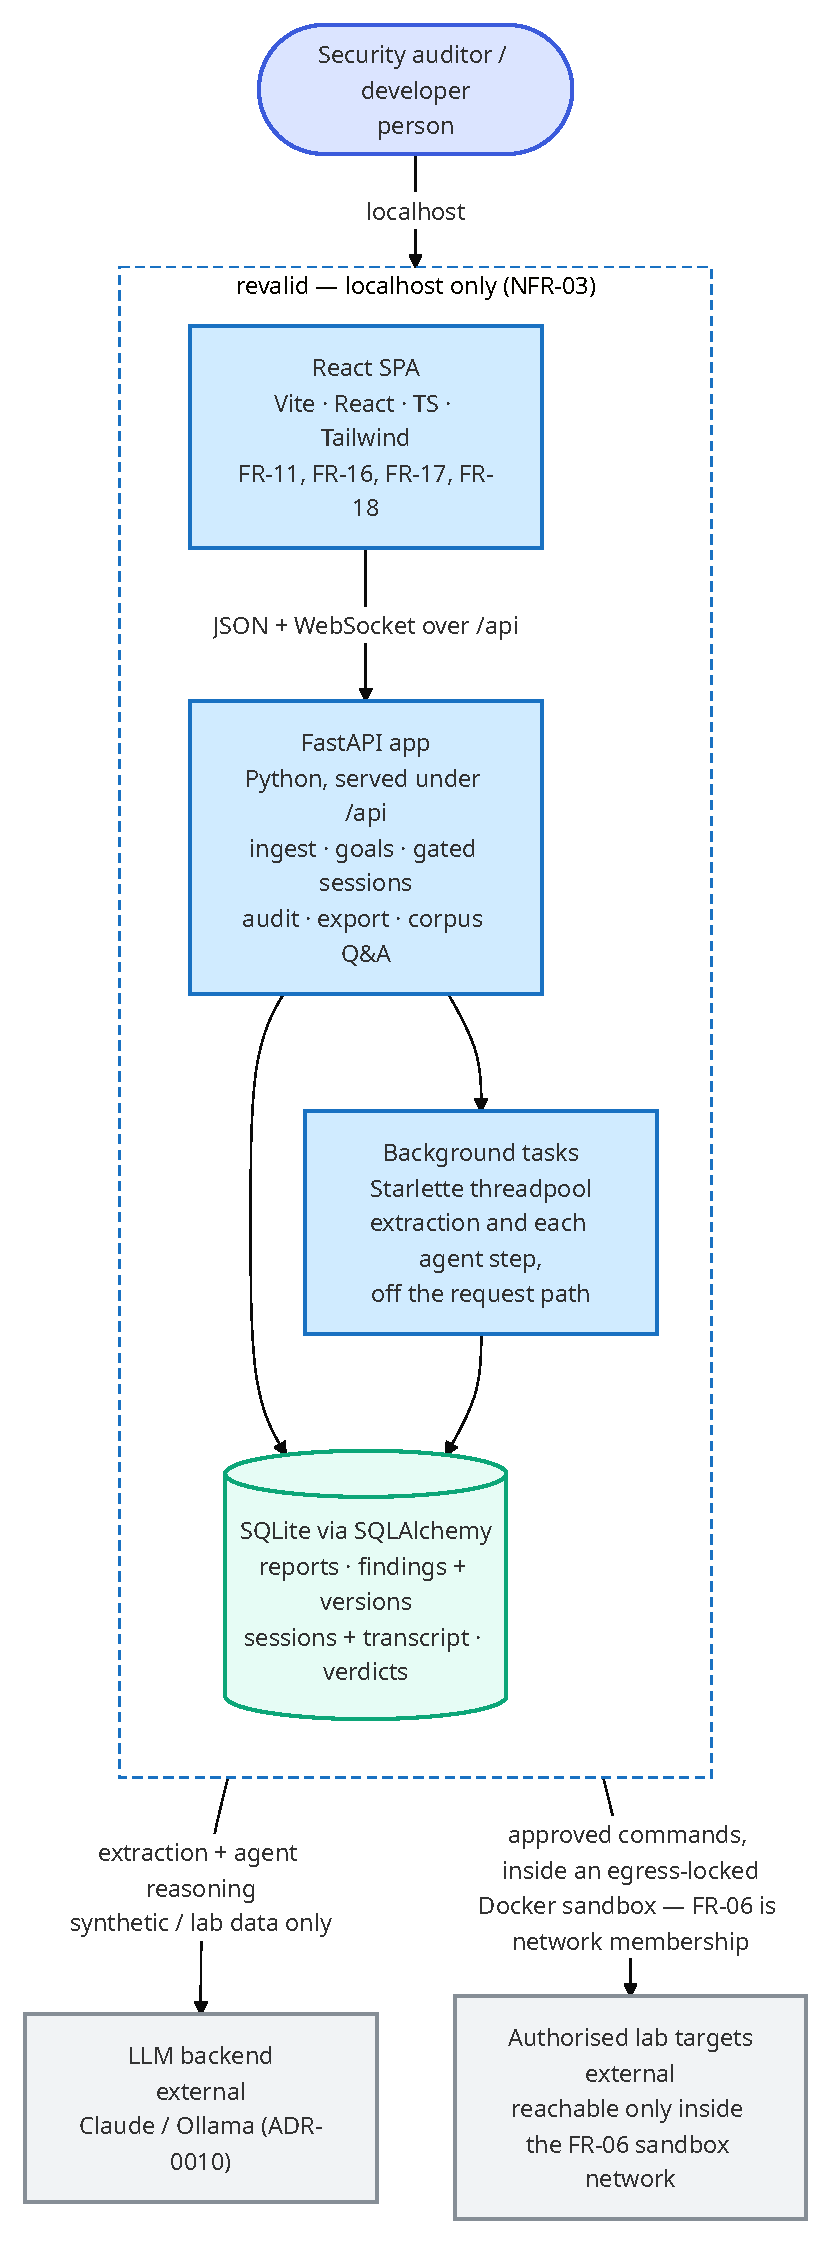
\includegraphics[height=0.62\textheight]{figs/arch-containers.pdf}
\caption[Container view]{The container view. Everything inside the dashed
boundary is one operating-system process bound to the loopback interface
(NFR-03). The interface talks to the API over JSON and, during a retest, a
WebSocket; approved commands reach the target only from inside the egress-locked
sandbox.}
\label{fig:arch-containers}
\end{figure}

There is no message broker, no worker fleet and no separate database server, and
their absence was argued rather than assumed. The alternative --- a queue and a
worker process --- buys durability of in-flight work across a restart, and costs
an operator two more things to install and keep running. For a tool whose unit of
work is an interactive session a human is watching, that trade is poor: if the
process dies mid-session the human is present to notice, whereas a broker that
must be running before the tool starts is a permanent tax on every use. The cost
of that choice is real and is paid in Section~\ref{sec:design-retest}: a retest
session lives partly in memory, so a restart abandons it.

\section{Backend decomposition}
\label{sec:design-components}

Figure~\ref{fig:arch-components} opens the backend container. Each box is a
Python module and each arrow is a real import, which makes the diagram checkable:
it is generated from the same source the documentation publishes, and a
dependency drawn here that does not exist in the code is a bug in the drawing.

\begin{figure}[!htb]
\centering
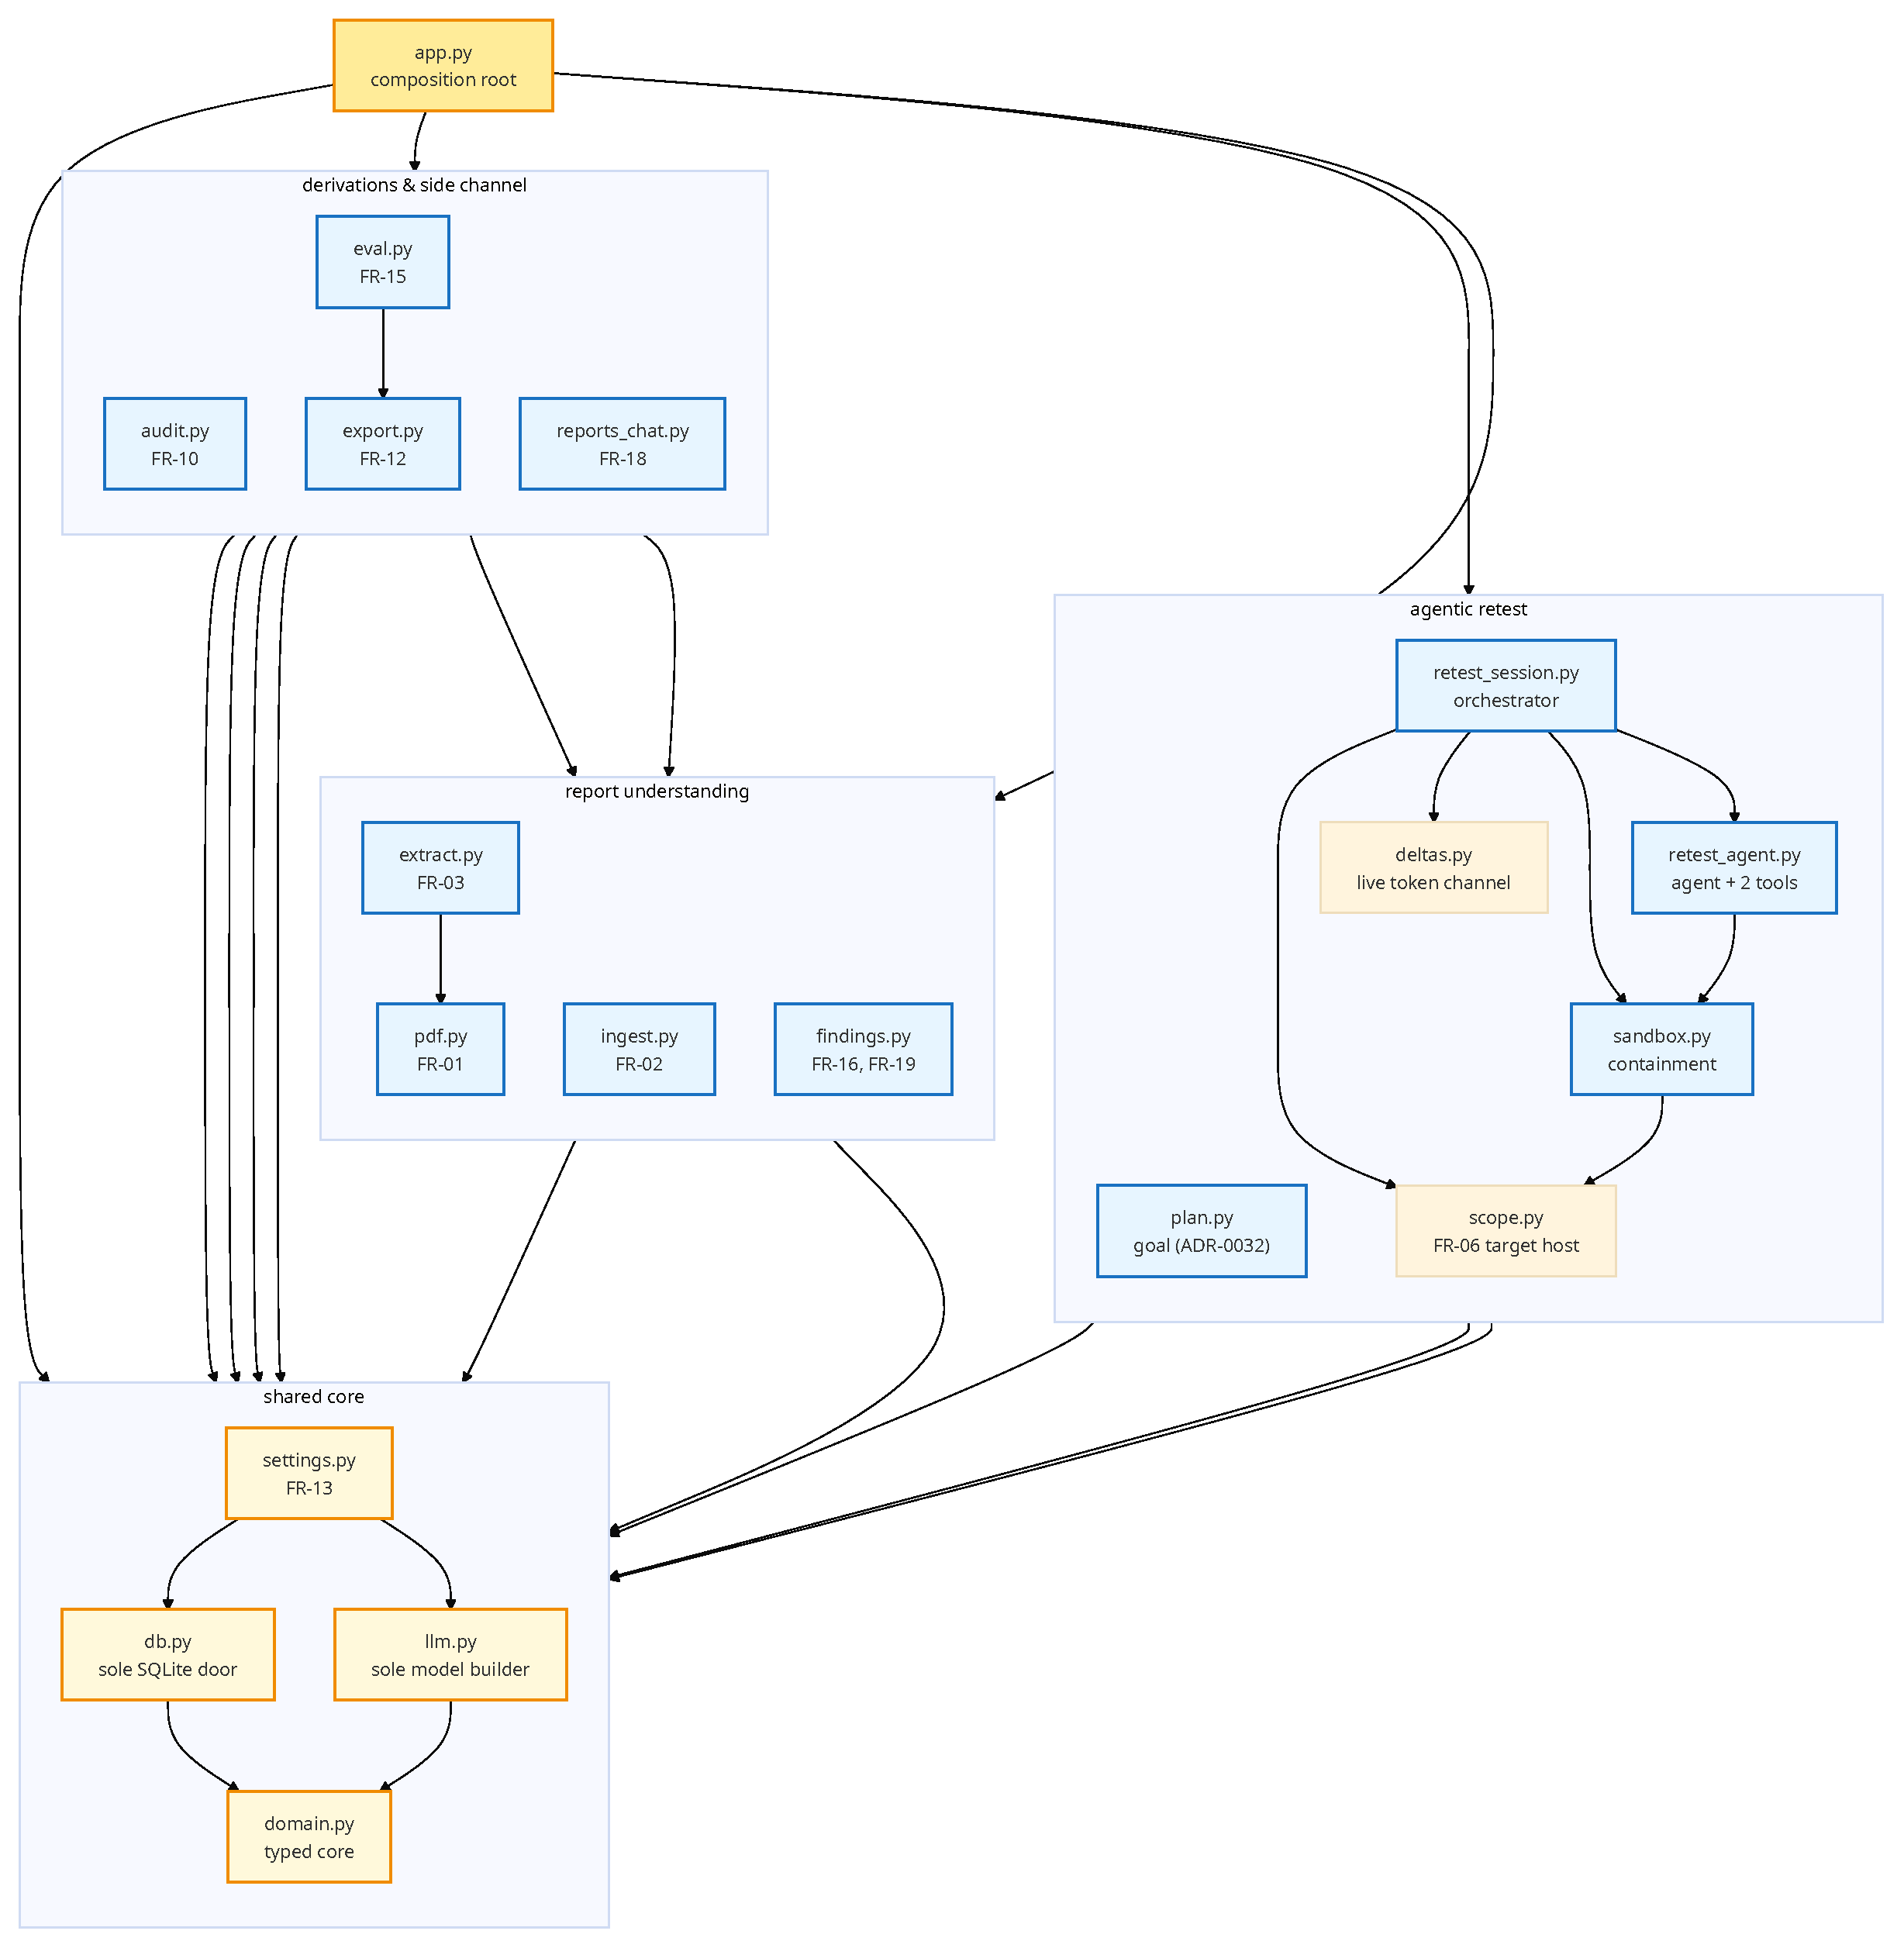
\includegraphics[width=\textwidth]{figs/arch-components.pdf}
\caption[Component view of the backend]{The backend modules and their real import
edges, grouped by concern. \texttt{app.py} is the composition root: it owns the
routes, wires every dependency and schedules background work. Arrows to
\texttt{domain.py} are omitted --- every module imports it.}
\label{fig:arch-components}
\end{figure}

Three invariants hold this structure together, and each is worth more than the
grouping itself.

\paragraph{The typed core depends on nothing.} \texttt{domain.py} contains the
finding, the verdict, the session states and the enumerations, and imports no
other module of the system. Everything else may depend on it; it depends on
nothing. This is what keeps the domain vocabulary from acquiring a database
shape or a web-framework shape, and it is the reason the persistence layer could
be reorganised twice --- once to version findings, once to collapse the verdict
model --- without the domain types moving.

\paragraph{One door to the schema.} \texttt{db.py} is the only module that
defines a mapped class or opens a database engine; every other module receives an
already-open session and works exclusively through those classes. No module
writes SQL of its own and none constructs its own connection. The benefit is not
purity but auditability: the persisted shape of the system has exactly one
definition, so a question like ``what columns does a verdict have?'' has a single
answer, and the two reorganisations described in
Section~\ref{sec:design-evolution} each touched one file.

\paragraph{One place a model is constructed.} \texttt{llm.py} is the only module
that builds a language-model client. Every agent --- extraction, goal generation,
the retest agent, the corpus assistant --- receives its model rather than
choosing one. That single choke point is what makes FR-13's promise real: the
backend is swapped from the settings view at runtime, and no component knows
whether it is talking to a hosted model or one running on the operator's own
machine.

\section{Runtime and containment}
\label{sec:design-runtime}

Figure~\ref{fig:arch-deployment} shows the same system as processes, files and
networks. It is the figure that carries the safety argument, because in this
design the topology \emph{is} the control.

\begin{figure}[!htb]
\centering
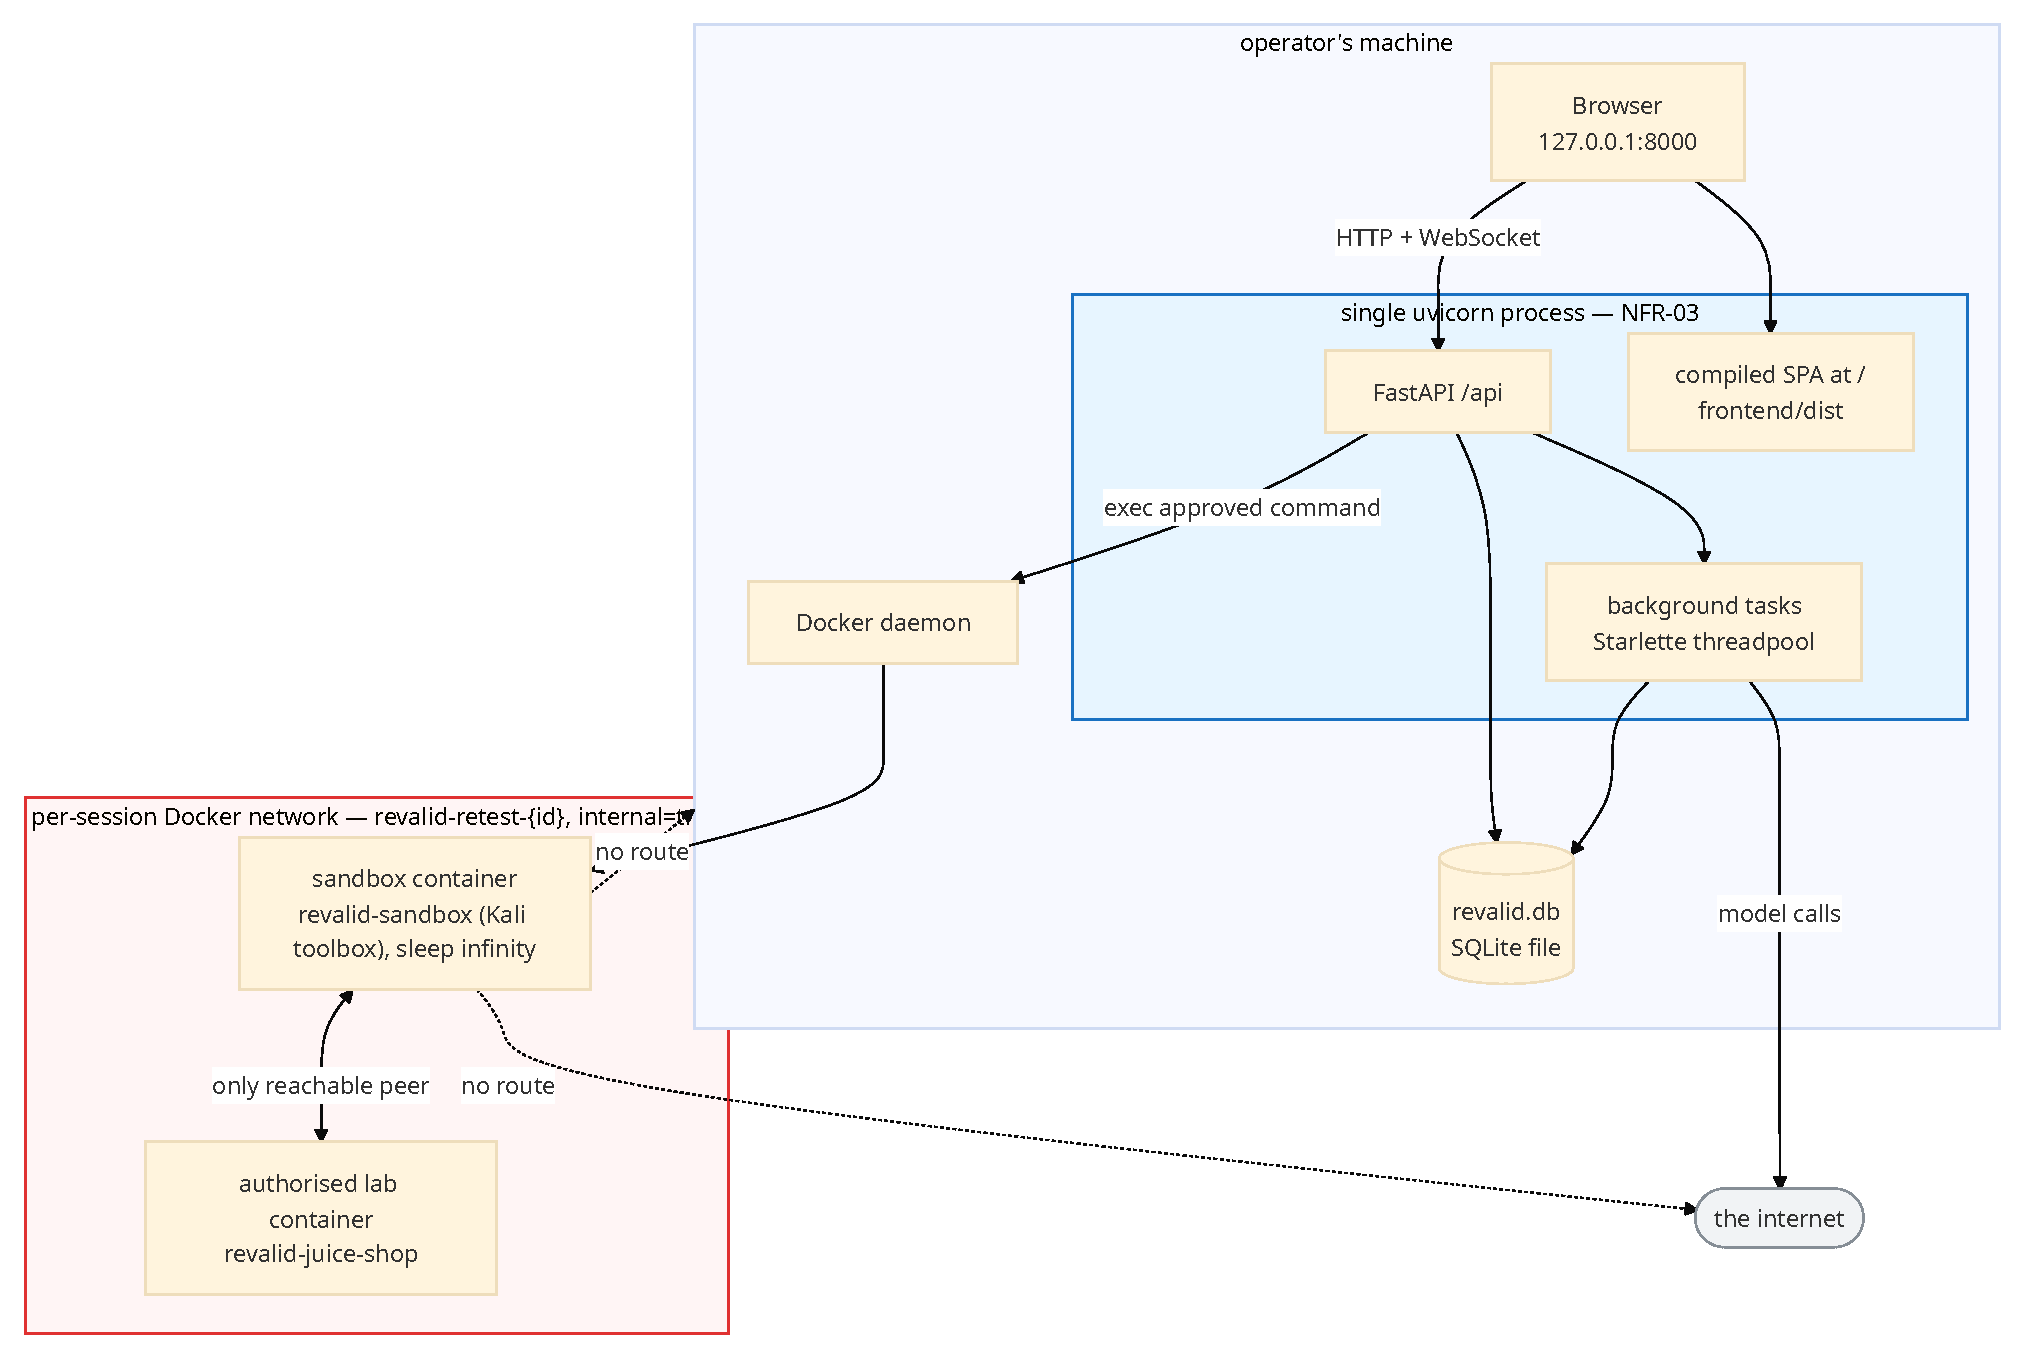
\includegraphics[width=\textwidth]{figs/arch-deployment.pdf}
\caption[Deployment and network topology]{Runtime topology. Dashed edges are
connections that \textbf{do not exist}: the per-session Docker network is created
in \texttt{internal} mode, so it has no gateway and the sandbox can reach neither
the host nor the internet. The lab container is the only other member of that
network, and therefore the only host the agent can reach.}
\label{fig:arch-deployment}
\end{figure}

The mechanism and its honest limits were set out in Section~\ref{subsec:stack} and
are not repeated here. What belongs in a design chapter is the reasoning behind
the shape. An authorisation rule can be expressed in two places: in the program,
as a check performed before each action, or in the environment, as an arrangement
in which the forbidden action has no meaning. The first is easier to write and
easier to test in isolation; it is also a promise that every future code path
must remember to keep, and it fails open when an address form is encountered that
its author did not anticipate. The second cannot be forgotten by a later change
to the agent, because it is not implemented in the agent at all.

This project began with the first design and moved to the second. That
migration, and the requirement it re-interpreted (FR-06), is one of the clearest
illustrations of the difference between a control that is stated and a control
that is enforced --- and it is why the deleted implementation is discussed rather
than quietly dropped.

\section{The data model}
\label{sec:design-data}

Figure~\ref{fig:arch-data-model} gives the persisted entities and their
relationships. The schema is small, and three of its properties carry most of the
design weight.

\begin{figure}[!htb]
\centering
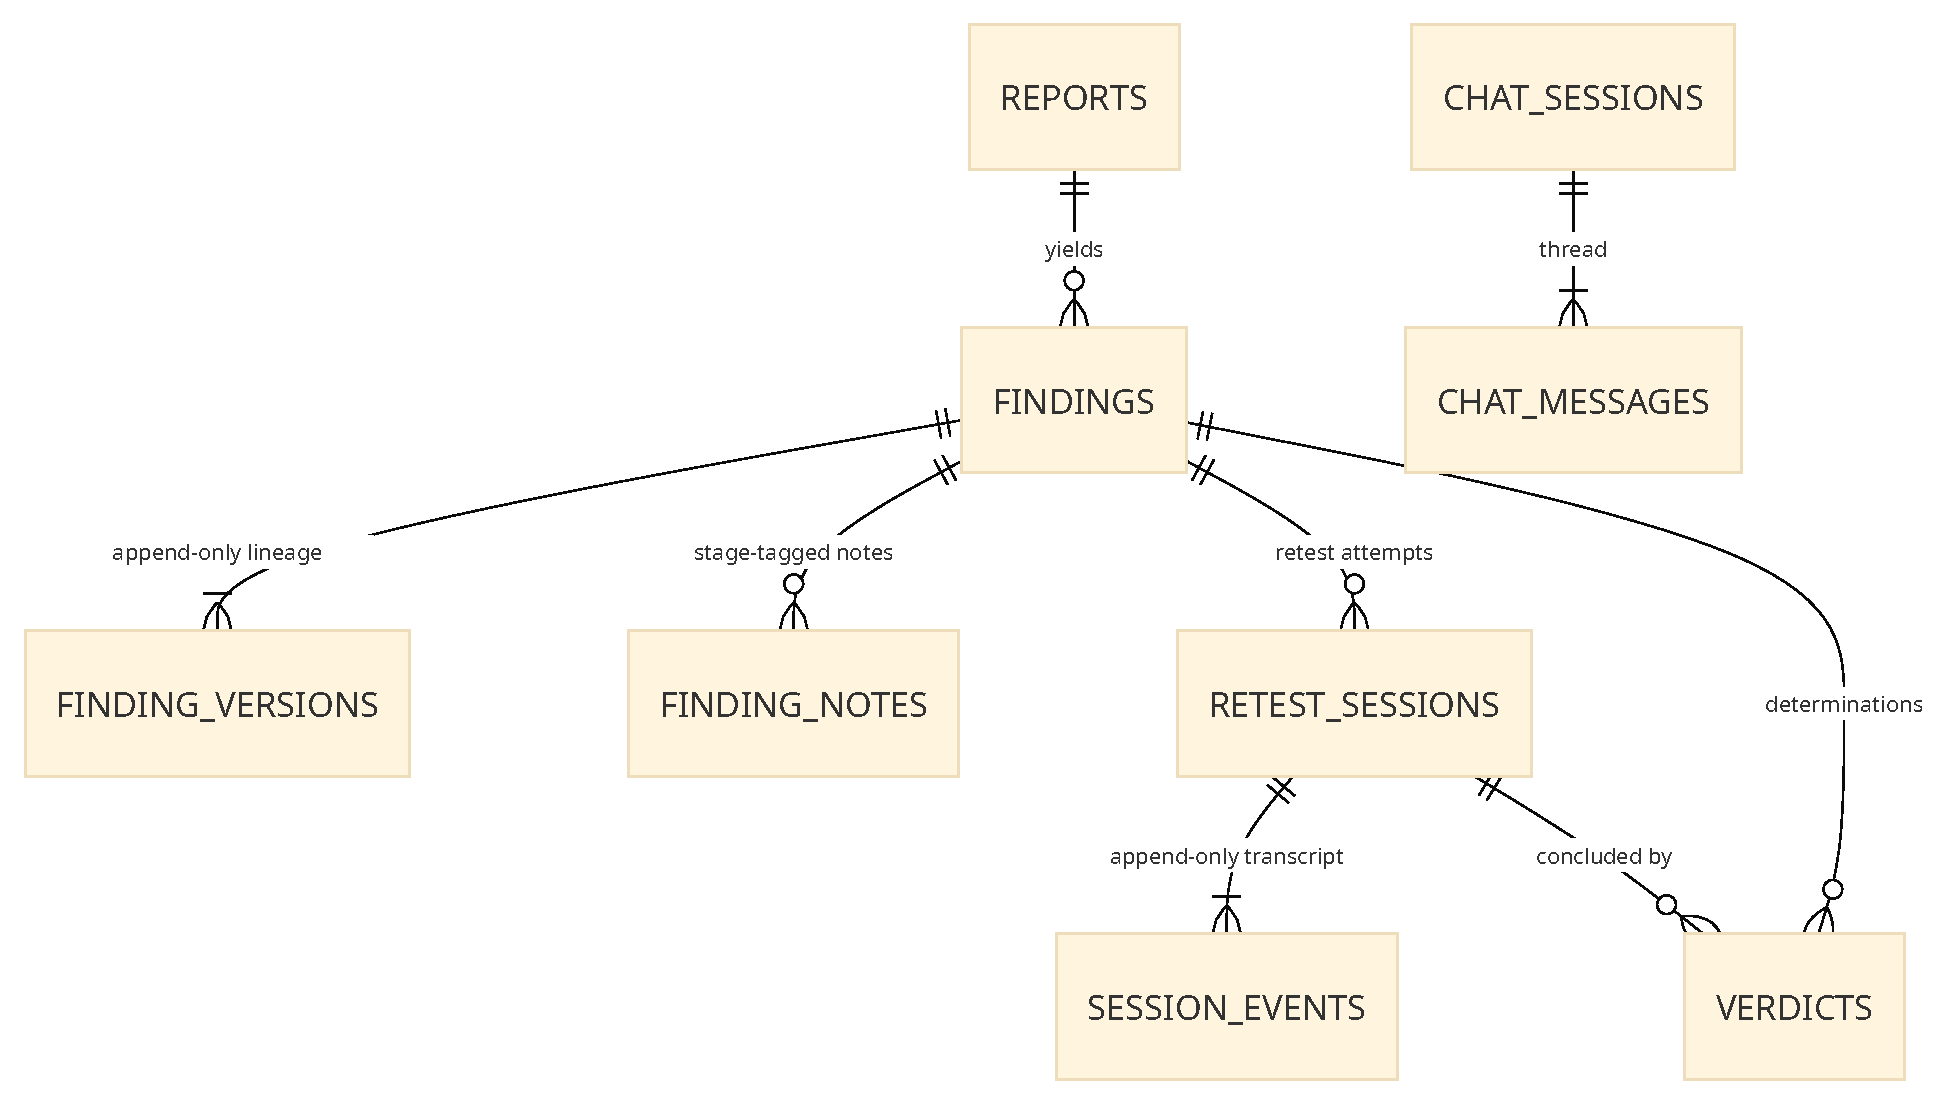
\includegraphics[width=\textwidth]{figs/arch-data-model.pdf}
\caption[Entity relationships]{The persisted entities. A report yields findings;
a finding owns an append-only chain of versions, its stage-tagged notes, its
retest sessions and its verdicts; a session owns its transcript. Chat threads are
independent of the rest.}
\label{fig:arch-data-model}
\end{figure}

\paragraph{A finding is an identity, not content.} The \texttt{findings} table
holds almost nothing --- an identifier and a link to the report it came from.
Every field a human reads lives in an append-only chain of versions, illustrated
in Figure~\ref{fig:arch-version-lineage}. Version one is always what the machine
proposed; each operator correction appends a new version with the reason it was
made, and nothing is ever overwritten.

\begin{figure}[!htb]
\centering
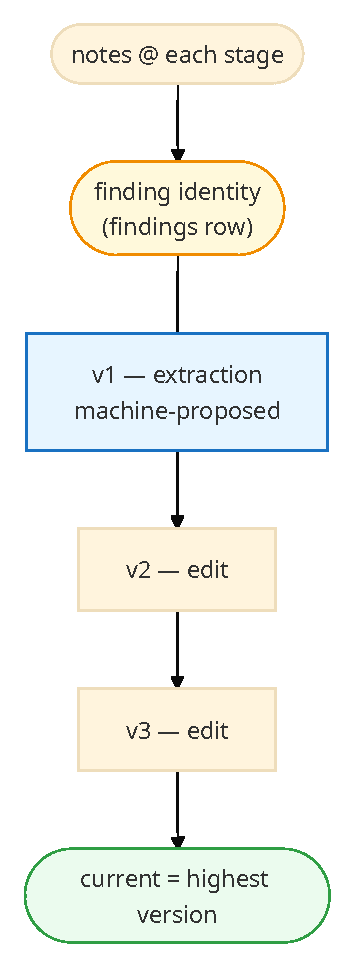
\includegraphics[width=\textwidth]{figs/arch-version-lineage.pdf}
\caption[Finding version lineage]{A finding's lineage. Version~1 is the
extraction --- what the model proposed. Each operator correction appends an
immutable version carrying the reason for the change, and the current view is
simply the highest. Notes attach to the stable identity and are tagged with the
pipeline stage on which they were written.}
\label{fig:arch-version-lineage}
\end{figure}

This is not archival fastidiousness. It is what makes the evaluation of
Chapter~\ref{ch:methodology}'s harness possible at all: measuring whether the
model extracted a finding correctly requires knowing what the model actually
said, \emph{after} a human has corrected it. A schema that let an operator edit a
finding in place would destroy the evidence needed to score the system --- the
correction would silently become the model's answer.

\paragraph{The transcript is the source of truth; the verdict is a derivation.}
A retest session owns an append-only, sequence-numbered transcript of everything
that happened in it. The verdict row is not the record of the outcome, it is a
denormalisation of the transcript event that announced the outcome. That ordering
is what FR-10 rests on, and it is the reason the audit of
Section~\ref{sec:design-derivations} can mean anything: a derived row can be
checked against the thing it was derived from, whereas a row that is its own
source cannot be checked at all.

\paragraph{The settings are a single row.} One authoritative record holds the
model, the provider address and the credential. It is seeded once from the
environment on a fresh database and is thereafter the only authority, so that the
question ``which backend produced this?'' has exactly one answer at any moment.
Each report and each session additionally records the model that served it, so
the answer survives a later change.

\section{The agentic retest loop}
\label{sec:design-retest}

This is the heart of the system, and the place where the thesis's claim ---
autonomy that accelerates an expert without replacing their judgement --- is
either true or merely asserted.

\subsection{Gating as a structural property}

The agent has exactly two tools. One, \texttt{respond}, lets it speak to the
operator in prose and touches nothing. The other, \texttt{run\_command},
executes a shell command in the sandbox and is declared as a \emph{deferred}
tool: the framework will not execute its body until an explicit approval is
supplied. A proposal therefore cannot resolve on its own. The agent's turn ends,
the run returns a request for a decision, and nothing has happened to the target.

The distinction from a conventional guard is worth stating plainly, because it is
the same distinction as in Section~\ref{sec:design-runtime}. A system that
executes the command and then checks whether it should have is safe only while
the check is correct and reachable. A system in which the execution path does not
exist without a human decision is safe by construction --- there is no ordering
of events, no exception, and no future refactor of the agent that produces an
unapproved command, because the approval is what supplies the tool's result.

Figure~\ref{fig:arch-gated-execution} traces one iteration.

\begin{figure}[!htb]
\centering
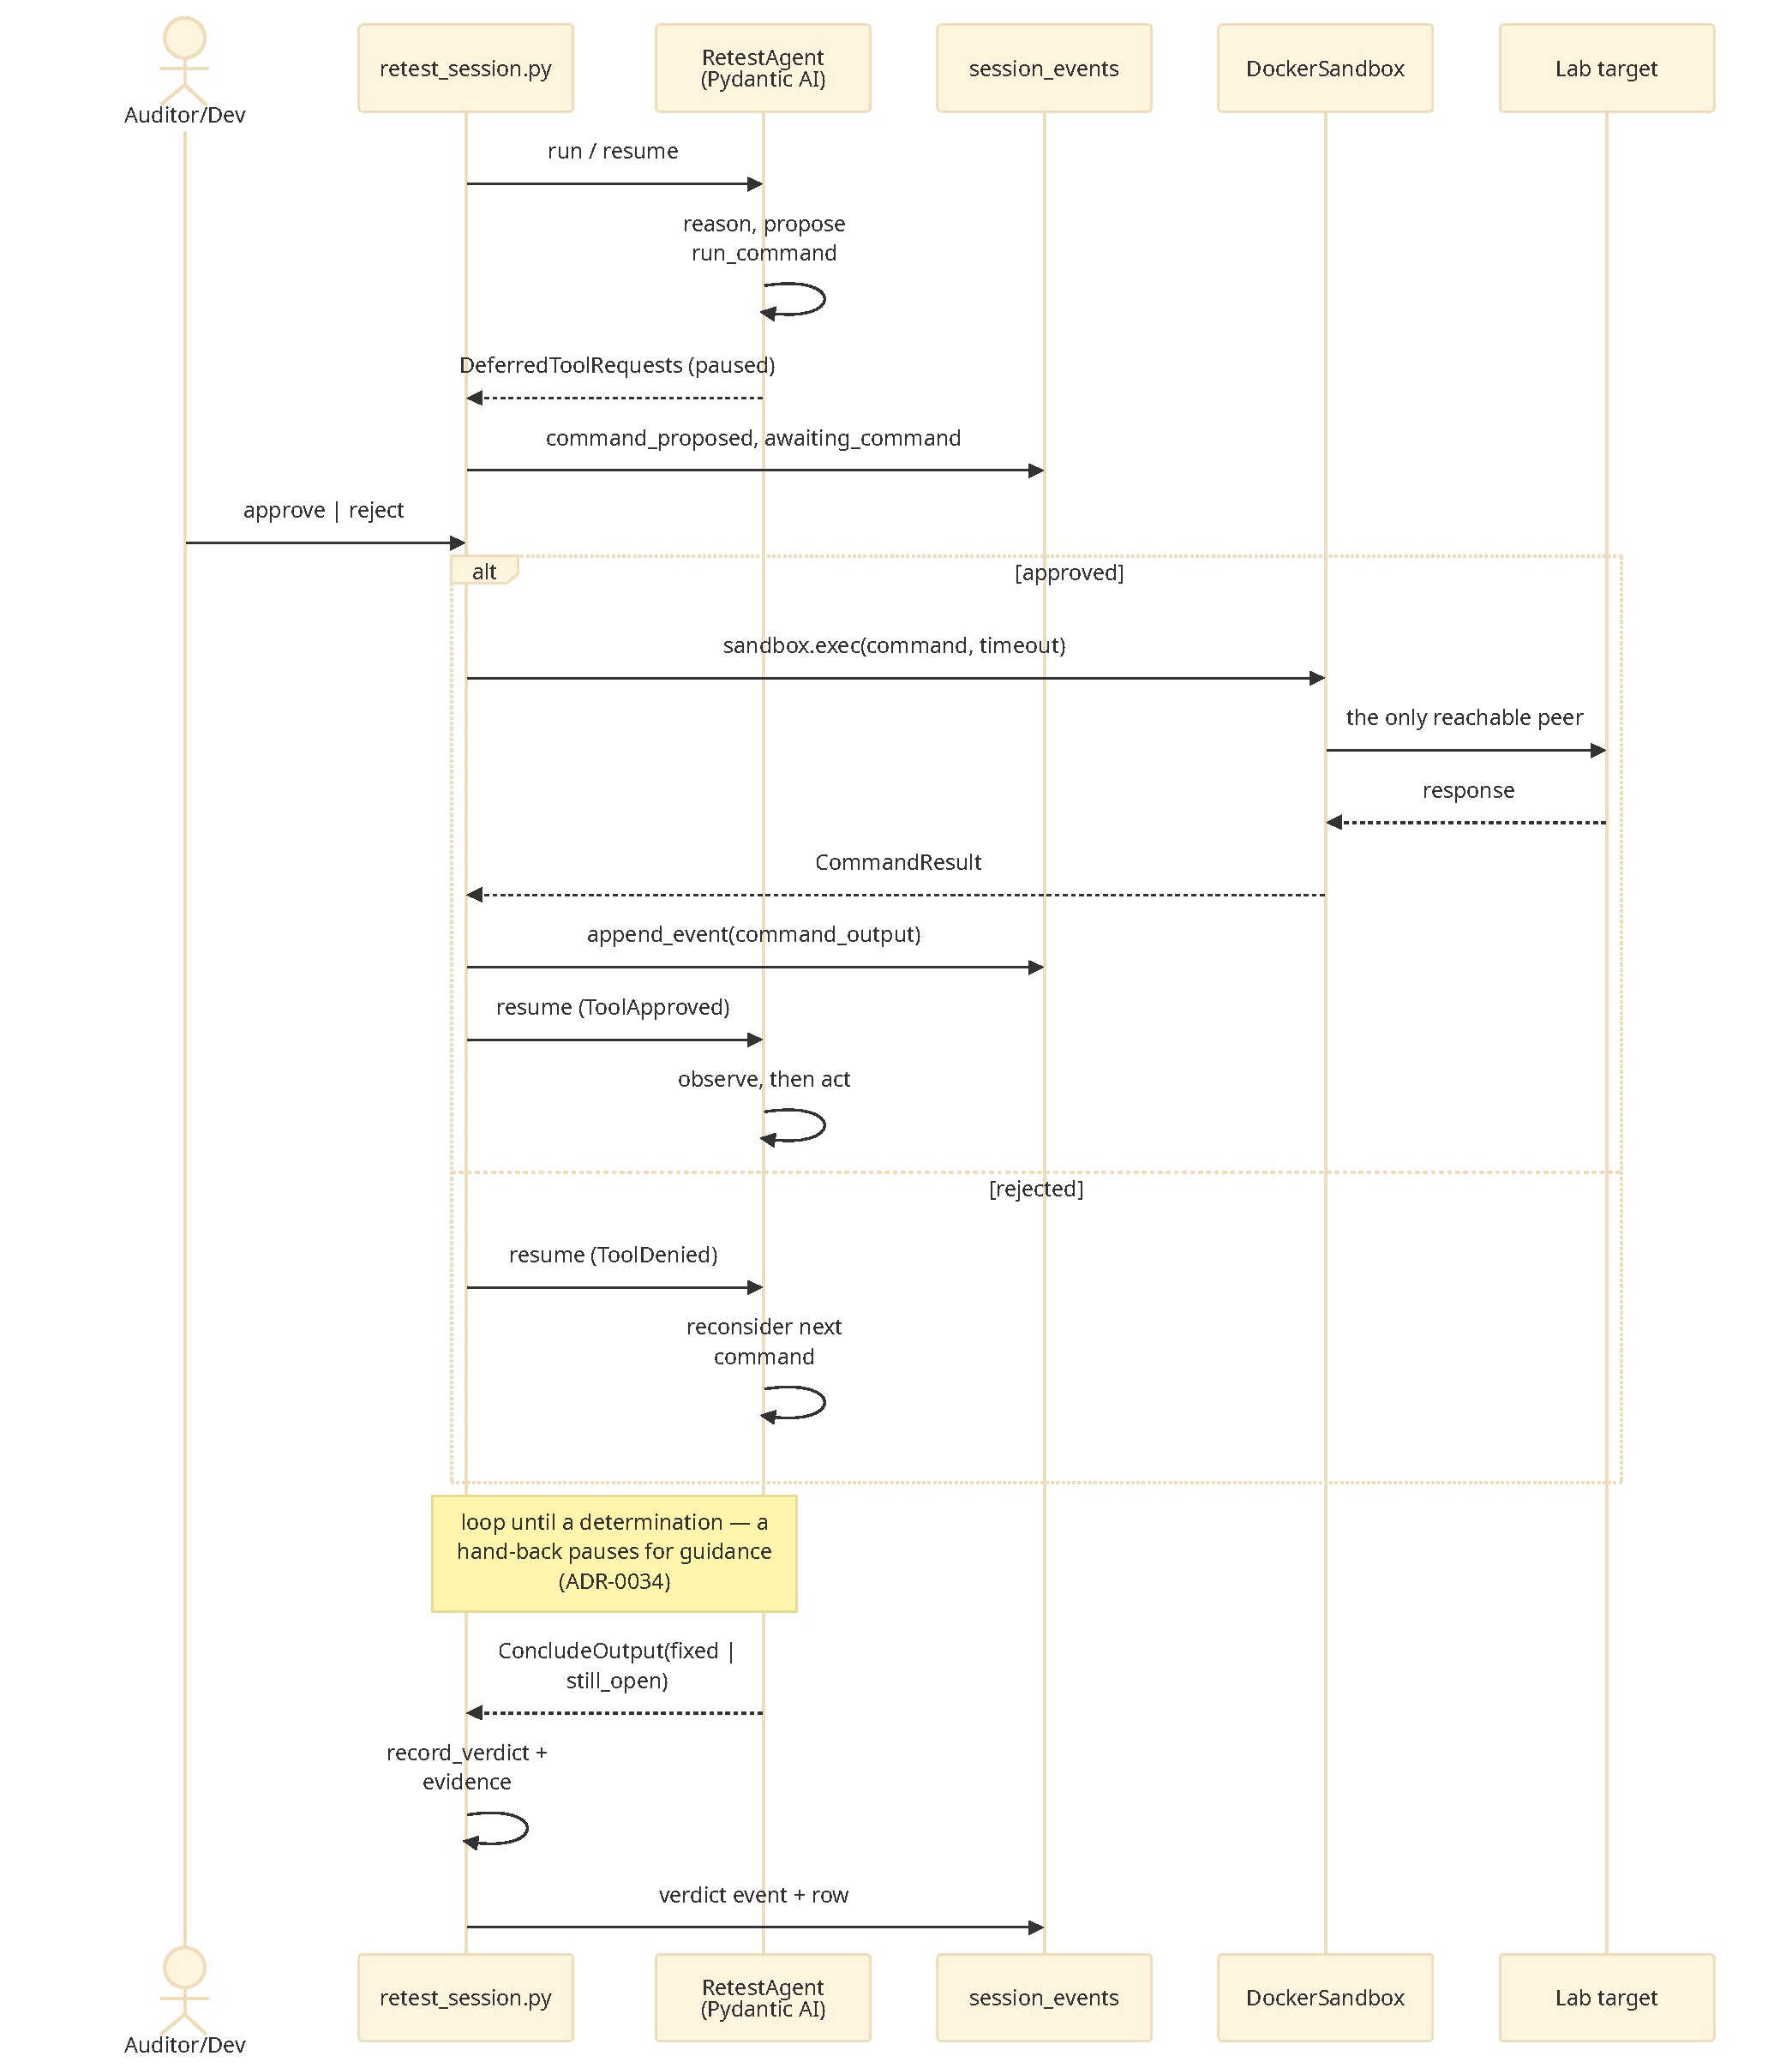
\includegraphics[height=0.74\textheight]{figs/arch-gated-execution.pdf}
\caption[One iteration of the gated retest loop]{The gated command cycle. The
agent reasons and proposes; the run pauses, unresolved, and the proposal is
appended to the transcript. Only after the operator approves does the command run
inside the sandbox, and only then is its real output returned to the agent as the
tool's result. A rejection resumes the agent with the denial and the operator's
reason, so a refusal is information rather than a dead end.}
\label{fig:arch-gated-execution}
\end{figure}

Two details of that cycle matter for the verdict's credibility. The output fed
back to the agent is the command's \emph{real} captured output --- exit status,
standard output and standard error --- not the agent's recollection of it; and
the same bytes are appended to the transcript, so the evidence a verdict cites is
the evidence the agent saw. A rejection is also not a dead end: the agent resumes
with the denial and the operator's stated reason, which lets a human steer by
refusing rather than by editing the agent's plan.

\subsection{The session lifecycle}

Figure~\ref{fig:arch-session-lifecycle} gives the states a session moves through.

\begin{figure}[!htb]
\centering
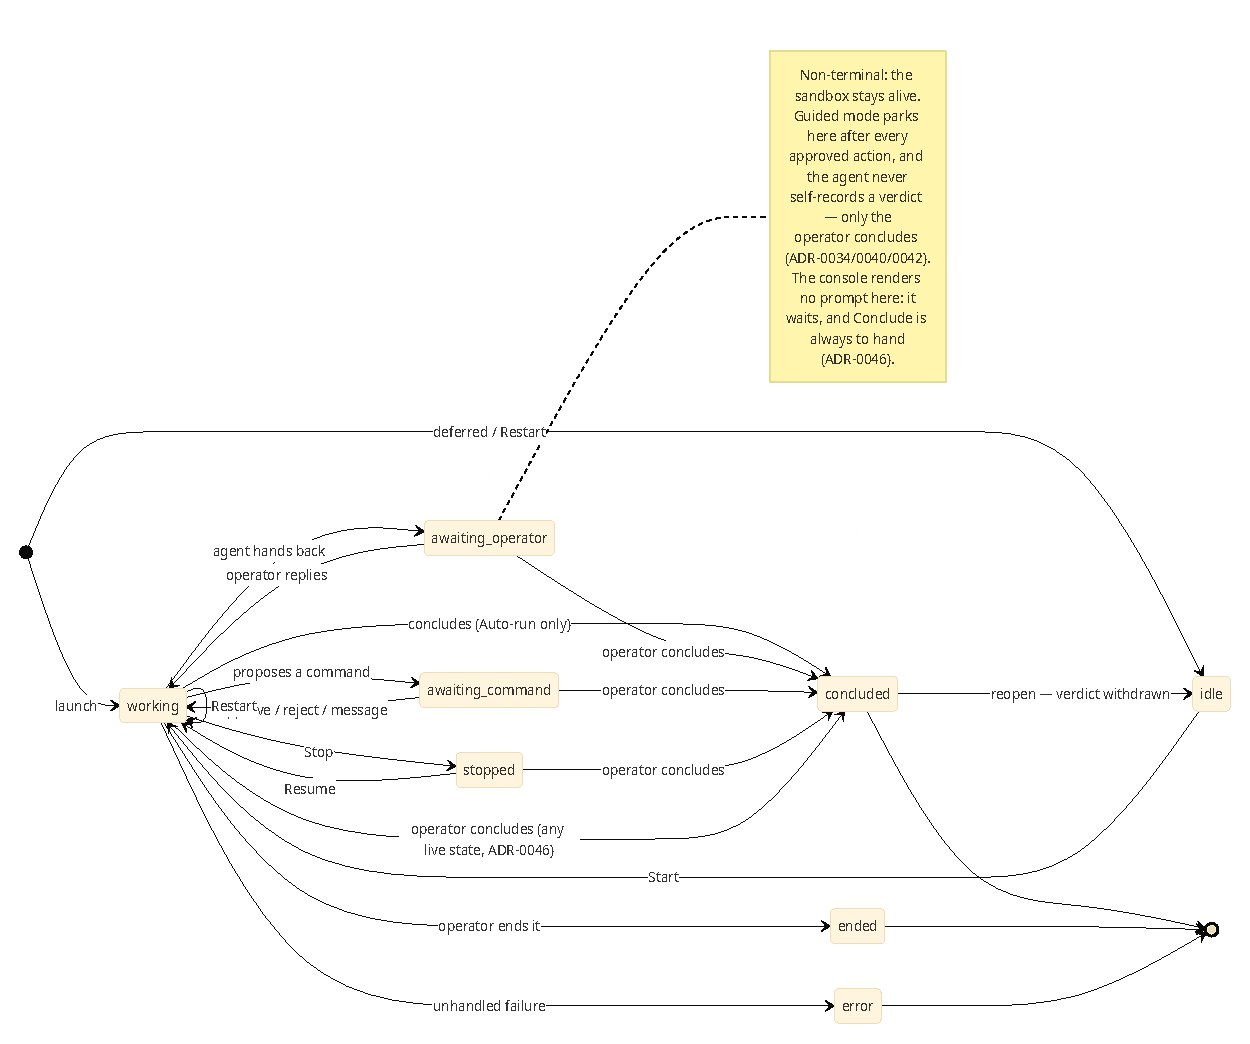
\includegraphics[height=0.55\textheight]{figs/arch-session-lifecycle.pdf}
\caption[Retest session lifecycle]{The session state machine. The loop between
\emph{thinking}, \emph{awaiting\_command} and \emph{running\_command} is the
gated cycle of Figure~\ref{fig:arch-gated-execution}. \emph{needs\_guidance} is
deliberately non-terminal: an agent that has run out of ideas hands the session
back to the operator instead of producing a verdict.}
\label{fig:arch-session-lifecycle}
\end{figure}

The most consequential state is \texttt{needs\_guidance}, and it exists because
of a failure mode specific to this problem. An agent that has exhausted its ideas
will, if the design demands a verdict, produce one --- and the verdict it
produces will be \emph{fixed}, because failing to reproduce a vulnerability looks
exactly like the vulnerability being gone. That is the single most damaging error
this system can make: a still-exploitable finding marked remediated, with an
evidence trail that reads as diligent. The design therefore refuses to let
``I could not reproduce it'' become a determination. The session pauses, keeps
its sandbox alive, and asks the operator to steer or to conclude manually. An
earlier design bounded the agent's effort with a step budget and treated
exhaustion of that budget as a give-up state; it was removed in favour of this
one. ADR-0034 first retired the give-up state, leaving the budget to pause rather
than terminate a session; ADR-0035 then removed the budget itself, on the grounds
that a step meter reads to an operator like a broken progress bar and is redundant
once the agent's own hand-back is a trigger. What remains is a single, meaningful
cause: the agent says it has run out of ideas.

A session is also not wholly durable, which is the cost promised in
Section~\ref{sec:design-overview}. Its transcript, status and goal are persisted,
but the live agent, its message history and its sandbox handle are held in an
in-memory registry, so a backend restart abandons an in-flight session: the row
survives in a non-terminal state and the sandbox has to be reclaimed separately.
That is the price of the broker-free design, and it is bounded precisely because a
session is something a human sits through rather than a job left to run unattended.

\subsection{Steering, and the shape of operator control}

Control is exercised in four ways, in increasing order of intervention: approving
or rejecting each proposed command; typing a message that reaches the agent as a
first-class turn on its next decision; editing the retest goal that frames the
whole session; and running a command directly in the same sandbox, which the
agent then observes on its next turn. The last of these is deliberately
\emph{not} gated. The gate exists to keep a machine from acting unilaterally, not
to supervise the human, and a tool that asked the operator to approve their own
command would be ceremony rather than safety.

A mode called \emph{free launch} removes the per-command approval and lets the
agent proceed on its own. It is included honestly and it is a real weakening of
the central claim: with it enabled, the system is an autonomous testing agent of
the kind Chapter~\ref{ch:sota} surveys, and its containment rests entirely on the
topology of Section~\ref{sec:design-runtime} rather than on human judgement.

\section{Derivations off the trail}
\label{sec:design-derivations}

Two read-only capabilities are built on the persisted transcript, and neither
touches the network.

The first is the FR-10 audit. For every stored verdict it re-projects the
authoritative transcript event --- the agent's own \texttt{verdict} event, or the
latest operator adjudication if the human overrode it --- and compares that
projection against the stored row. A clean run establishes that no verdict has
drifted from the trail it was derived from. It is important to be exact about
what this does and does not establish, since the vocabulary invites
over-reading: it verifies the integrity of a denormalisation, not the soundness
of the agent's reasoning. Whether the agent was \emph{right} is an empirical
question about outputs, answered by the evaluation harness against ground truth,
not by re-reading the record.

The second is the FR-12 export: a single versioned JSON document containing the
reports, findings with their version history and notes, and the verdicts with
their evidence. Its schema is \emph{generated} from the same models that produce
the document and published alongside it, with a test that fails if the published
schema and the generated one diverge --- the same principle as the figures in
this chapter, applied to a data contract. The evaluation harness consumes that
document, which is what allows scoring to happen offline, on a file, without a
live system.

\section{How the design changed}
\label{sec:design-evolution}

The system described so far is the second architecture this project built. The
first worked, was tested, was documented, and was deleted. Reporting only the
survivor would misrepresent both the effort involved and the reasoning that
produced the final design.

\paragraph{What the first design was.} A retest was a \emph{batch}. A language
model proposed a structured plan of typed probes; a deterministic gate bound each
probe to an authorised base address and discarded anything that failed a
request-level allowlist or used a destructive method; a human approved the plan
as a whole; an executor then ran the surviving probes over HTTP, captured request
and response evidence, and a set of rule-based assessors mapped that evidence to
a verdict with a machine-readable reason code. FR-04, FR-05, FR-07 and FR-08 are
that design, and FR-14 added a browser-driven executor for findings that only
reproduce in a real page.

\paragraph{Why it was replaced.} Two limitations emerged from using it. The first
was expressive: a plan fixed in advance cannot react. Real revalidation is
conditional --- an endpoint responds differently than the report described, a
credential has rotated, a payload needs one adjustment --- and a batch that
commits to its steps before seeing any of them either succeeds by luck or fails
without learning anything. The second was that the approval gate sat at the wrong
granularity. Approving a plan of eight probes is approving an intention;
approving each command as it is proposed, with the previous command's output
visible, is approving an action. Only the second is the kind of control the
system claims to offer.

\paragraph{What it cost, and what was kept.} Replacing it removed about
5{,}500 lines of working, tested code from the backend in one slice and a further
2{,}100 in the interface reshape that followed, together with five requirements'
worth of implementation. It was done in deliberate slices, with the old path kept
operational until the new one was complete. Two things were kept rather than
rebuilt. The evidence-backed verdict of FR-09 survived, with its shape
generalised so that proof could come from an arbitrary command's real output
rather than from a structured HTTP exchange. And FR-06 survived in the strongest
sense: its \emph{requirement} was retained while its \emph{implementation} moved
from a request-level allowlist into the network topology, which is how a
capability that was previously a promise inside the program became a property of
the environment.

\paragraph{The judgement.} The batch design was not a mistake, and it is not
presented as one. It was the correct first architecture: deterministic, easy to
reason about, and the only sensible way to establish that a language model could
be constrained enough to be trusted with a security decision at all. What it
could not do was represent the interaction a revalidation actually is. The
decision to delete it was taken only once the agentic path covered the whole
retest lifecycle end to end on the same lab targets, and it was recorded --- with
its rationale, its alternatives and its consequences --- in ADR-0033, which
supersedes the eight architecture decision records the batch path rested on. That
record is the most accurate surviving artefact of the *reasoning* this chapter
describes, which the remaining code cannot show.
